\documentclass[12pt]{article}

\usepackage{float}
\usepackage{amsmath}
\usepackage{graphicx}
\usepackage{enumitem}
\usepackage[margin=1.50in]{geometry}
\usepackage[font=footnotesize]{caption}

\usepackage{bm}
\newcommand{\m}[1]{\mathbf{\bm{#1}}}

\usepackage{natbib}
\bibpunct{(}{)}{;}{a}{}{,}

\begin{document}

\begin{LARGE}
\noindent Dirichlet process mixture model on Hopkinson-bar experiments
\end{LARGE}
\bigskip

\noindent Mickey Warner

\noindent AMS 241

\section{Introduction}

Hopkinson-bar (or Split-Hopkinson pressure bar) experiments are compression tests performed on small (e.g. 6.35mm diameter plates) samples of materials. The material undergoes a deformation which is measured by a strain-stress ($\epsilon$-$\sigma$) response. Strain measures changes in the length of the material, and stress measures changes in the cross-sectional area. A single experiment yields a strain-stress curve.

An experiment may fall within two classes of tests: quasi-static or dynamic. In quasi-static tests, the compression occurs very slowly, attempting to measure infinitesimal changes in the response. These are associated with low strain rates, $\dot\epsilon$. Dynamic tests occur at high strain rates and are characterized by higher volatility in the response curve.

Other variations of this experiment exist, but the data we will look at in this paper come from either quasi-static or dynamic tests. The data are of Hopkinson-bar tests performed on samples of tantalum by \cite{chen1996constitutive} (see figure \ref{data}), at various strain rates and initial temperatures.

The goal is to model these response curves so we can make accurate predictions for future experiments. The curves themselves (and consequently any predicted curve) may be fed into more complicated materials science models such as those involving 3-D printing. Materials models have been developed to capture the physics and behavior of Hopkinson-bar experiments. We will use a simplified version of a particular model, the Johnson-Cook model, in conjunction with a Dirichlet process mixture model, as our statistical model.

In section 2, we discuss some of the ideas used in modeling these kinds of experiments, from both materials science and statistics perspectives. We discuss Dirichlet process mixture models in section 3 and provide an example of its usage to a simulated data set in section 4. In section 5 we analyze the Hopkinson-bar tests from \cite{chen1996constitutive}. We conclude in section 6 with a discussion.

\begin{figure}[H]
\begin{center}
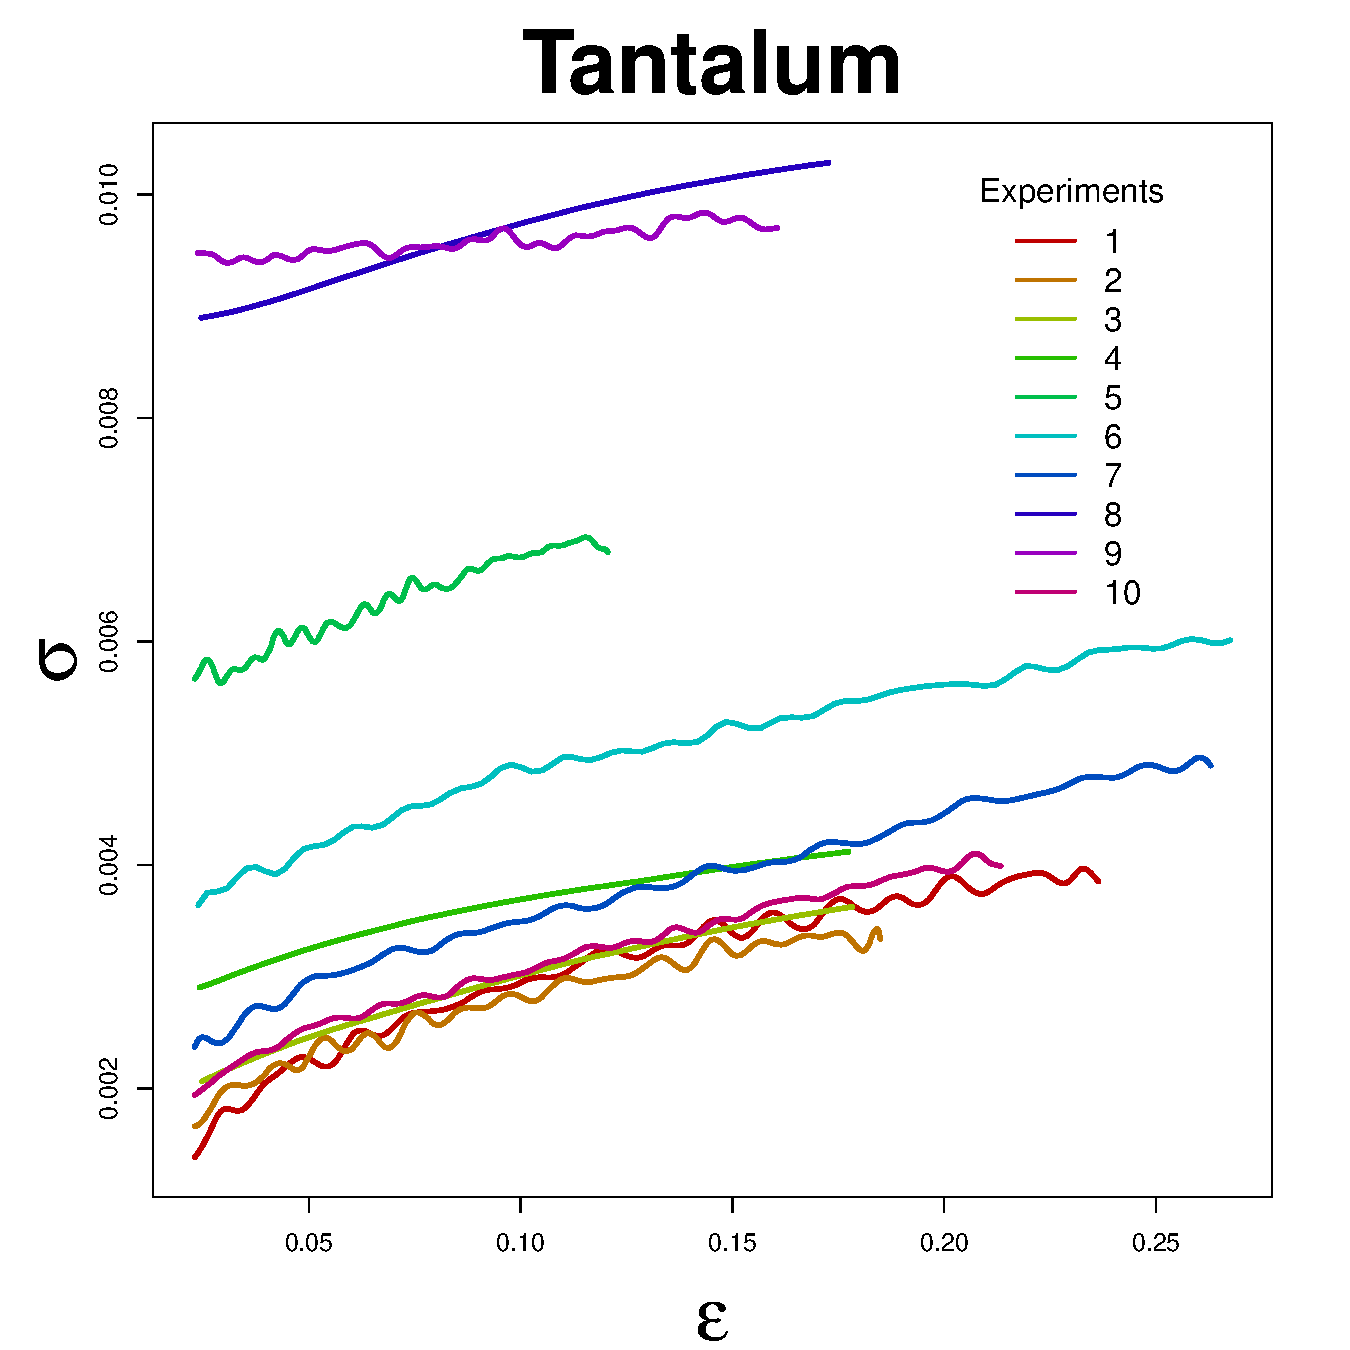
\includegraphics[scale=0.40]{../figs/ta_all_data.pdf}
\caption{Strain-stress response from ten experiments at various strain rates and temperatures.}
\label{data}
\end{center}
\end{figure}

\section{Brief review of current approaches}

Perhaps the simplest materials model that attempts to model the stress $\sigma$ is the Johnson-Cook model:
\begin{align}
\m{\sigma}(\m{x}, \m{\theta}) = (A+B\epsilon_p^n)(1+C\log\dot\epsilon)(1-T^m)
\label{jc}
\end{align}
where $\m{x}$ encodes the plastic strain $\epsilon_p$ (the $x$-axis in figure \ref{data}), strain rate $\dot\epsilon$, and scaled temperature $T$ for a specific experiment, and $\m{\theta}=(A,B,n,C,m)$ is the vector of parameters to be estimated. Other models exist that may have more parameters, and hence better predictive capabilities, but model (\ref{jc}) provides us with a convenient starting point.

A typical approach in the materials science community is to assume a common $\m{\theta}$ among all experiments and then minimize some goodness-of-fit function. The minimization may be done by optimizing one parameter at a time, holding some parameters fixed (for more complicated models), or even by looking at a graph. We would at least prefer a systematic method of estimating the parameters.

A challenge for any materials model is the potential lack in accurately accounting for all of the necessary physics in the experimental procedure. If a key component is missing, predictions made at untried experimental settings may fail. If too many terms are added, we run the risk of overfitting.

\cite{fugate2005hierarchical} fit a hierarchical Bayesian model to Hopkinson-bar experiments. By assuming each experiment has its own $\m{\theta}_i$, the authors found that the added flexible increased the predictive power of the statistical model. A model with common $\m{\theta}$ yielded predictive uncertainty that was too conservative. In the hierarchical setting, the mean predictive curve for a new experiment was more accurate, but the predictive variance necessarily increased.

A parametric assumption made by \cite{fugate2005hierarchical} is that the population distribution for the $\m{\theta}_i$'s is (truncated) multivariate normal. For data sets or materials models where the random effects $\m{\theta}_i$ do not come from a normal distribution, predictions based on this hierarchical model do very poorly.

\section{Dirichlet process mixture models}

The Dirichlet process mixture model assumes a non-parametric prior on the distribution of random effects.

\section{Simulation example}

\section{Analysis of the Hopkinson-bar experiments}

\section{Discussion}

% 
% \begin{itemize}[label=$\cdot$]
% \item
% \end{itemize}
% 
% \begin{center}
% \begin{tabular}{lrrrrrr}
%          &      & \multicolumn{5}{c}{Quantiles} \\
%          & Mean & \multicolumn{1}{|r}{0\%}  & 2.5\% & 50\% & 97.5\% & 100\% \\ \hline\hline
% $\alpha$ & 2.64 & 0.00 & 0.23 & 2.02 & 8.50 & 24.50 \\ 
% $\beta$ & 0.19 & 0.01 & 0.10 & 0.18 & 0.27 &  0.36 \\
% $\zeta$ & 3.88 & 0.03 & 0.75 & 3.46 & 9.27 & 18.19 \\
% $\mu$   & 2.96 & 0.29 & 1.26 & 2.75 & 5.85 & 13.50 \\ \hline
% \end{tabular}
% \end{center}


\bibliography{refs}
\bibliographystyle{asa}


\end{document}
